\iffalse
\let\negmedspace\undefined
\let\negthickspace\undefined
\documentclass[journal,12pt,twocolumn]{IEEEtran}
\usepackage{cite}
\usepackage{amsmath,amssymb,amsfonts,amsthm}
\usepackage{algorithmic}
\usepackage{graphicx}
\usepackage{textcomp}
\usepackage{xcolor}
\usepackage{txfonts}
\usepackage{listings}
\usepackage{enumitem}
\usepackage{mathtools}
\usepackage{gensymb}
\usepackage{comment}
\usepackage[breaklinks=true]{hyperref}
\usepackage{tkz-euclide} 
\usepackage{listings}
\usepackage{gvv}                                        
\def\inputGnumericTable{}                                 
\usepackage[latin1]{inputenc}                                
\usepackage{color}                                            
\usepackage{array}                                            
\usepackage{longtable}                              
\usepackage{calc}                                             
\usepackage{multirow}                                         
\usepackage{hhline}                                           
\usepackage{ifthen}                                           
\usepackage{lscape}

\newtheorem{theorem}{Theorem}[section]
\newtheorem{problem}{Problem}
\newtheorem{proposition}{Proposition}[section]
\newtheorem{lemma}{Lemma}[section]
\newtheorem{corollary}[theorem]{Corollary}
\newtheorem{example}{Example}[section]
\newtheorem{definition}[problem]{Definition}
\newcommand{\BEQA}{\begin{eqnarray}}
\newcommand{\EEQA}{\end{eqnarray}}
\newcommand{\define}{\stackrel{\triangle}{=}}
\theoremstyle{remark}
\newtheorem{rem}{Remark}
\begin{document}

\bibliographystyle{IEEEtran}
\vspace{3cm}

\title{NCERT DISCRETE}
\author{EE23BTECH11214 - Harsha Vardhan Paramata$^{*}$% <-this % stops a space
}
\maketitle
\newpage
\bigskip

\renewcommand{\thefigure}{\theenumi}
\renewcommand{\thetable}{\theenumi}

\textbf{Question 10.5.4.1}:
Which term of the AP: 121, 117, 113, \ldots, is its first negative term?

% Solution
\textbf{Solution}:
\fi
\begin{table}[htbp]
\centering
\begin{tabular}{|l|l|c|}
\hline
\textbf{Symbol} & \textbf{Description} & \textbf{Value} \\
\hline
$x\sbrak{n}$ & General term & \(121 - 4n\) \\
\hline
$x\sbrak{0}$ & Initial term & 121 \\
\hline
$d$ & Common difference & 4 \\
\hline
\end{tabular}

\caption{parameters list}
\end{table}

\begin{align}
x\sbrak{n} &= 121 - 4n < 0 \\
n &> \frac{121}{4} 
\end{align}
The first negative term in the sequence occurs at 
$n = 31$  \\
Z-transform of this sequence:
\begin{align}
    X\brak{z} &= \frac{121 - 125z^{-1}}{1 - 2z^{-1} + z^{-2}}
 ,\quad \abs{z} > \abs{1}
\end{align}
\begin{figure}[!ht] 
\centering
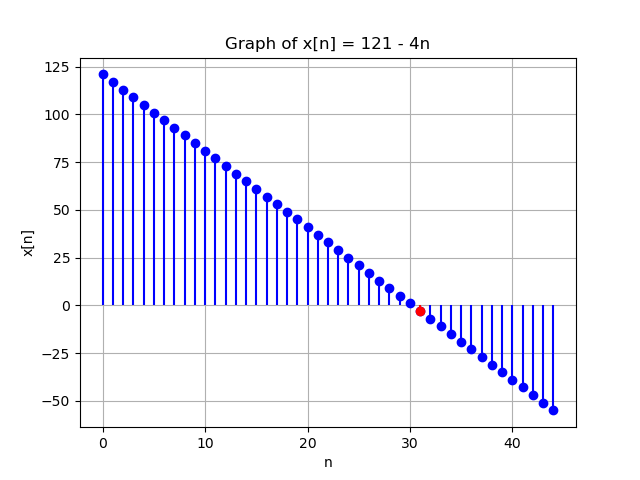
\includegraphics[width=1\columnwidth]{ncert-maths/10/5/4/1/figs/graph.png}
\end{figure}
%\end{document}
